\documentclass{beamer}
\usepackage{listings}
\usepackage{subfig}
\usepackage{bytefield}
\usetheme{metropolis}
\title{Wireguard: A Modern VPN Protocol}
\author{Jinank Jain, Rayhaan Jaufeerally}
\institute{ETH Z\"urich}
\begin{document}
    \maketitle
    \section{Introduction}
    \begin{frame}{Why VPN?}
        \begin{itemize}
            \item Necessary for point to point security between campuses (e.g. DC's, corporate offices, \ldots)
                \begin{itemize}
                    \item As early as the 1970's governments have tapped undersea cables for intelligence,
                    \item Operation Ivy Bells in 1971 tapped Russian communicatioons to millitary bases\footnote{\url{https://en.wikipedia.org/wiki/Operation\_Ivy\_Bells}},
                \end{itemize}
            \item Necessary for end users to get a clean connection:
                \begin{itemize}
                    \item ISP's doing DNS hijacking to serve inappropriate content,
                    \item Open WiFi networks when travelling,
                    \item Geoblocking,
                \end{itemize}
        \end{itemize}
    \end{frame}
    \begin{frame}{Necessity in real life}
        \begin{figure}
            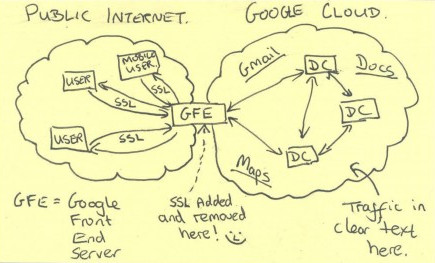
\includegraphics[width=\textwidth]{motivation.jpg}
            \caption{Nation state surveillance of user data including SPII.}
        \end{figure}
    \end{frame}
    \begin{frame}{History of VPN protocols}
        \begin{itemize}
            \item IPSEC
                \begin{itemize}
                    \item Popular for site to site connections with dedicated router hardware,
                    \item Tedious to set up and high degree of complexity,
                    \item Large attack surface between IKE (v2), SA mechanisms, XFRM in Linux,
                    \item Legacy protocol support,
                    \item IP in IP,
                \end{itemize}
            \item OpenVPN
                \begin{itemize}
                    \item Implemented in userspace with TUN/TAP (slow),
                    \item Complex confoguration vulnerable to leaks,
                    \item Stateful protocol which is brittle in real networks,
                    \item Large codebase / attack surface,
                \end{itemize}
        \end{itemize}
    \end{frame}
    \begin{frame}{What is Wireguard?}
        \begin{itemize}
            \item Opinionated Layer 3 secure network tunnel for IPv4 and IPv6.
            \item Lives in the Linux kernel, but cross platform userspace implementations are available.
            \item UDP based. Punches through firewall.
            \item Conservative and modern cryptographic principles.
            \item Emphasis on simplicity and single user auditability.
            \item Authentication model similar to SSH's \texttt{authorized\_keys}.
        \end{itemize}
    \end{frame}
    \begin{frame}{Easily Auditable}
        \begin{figure}
            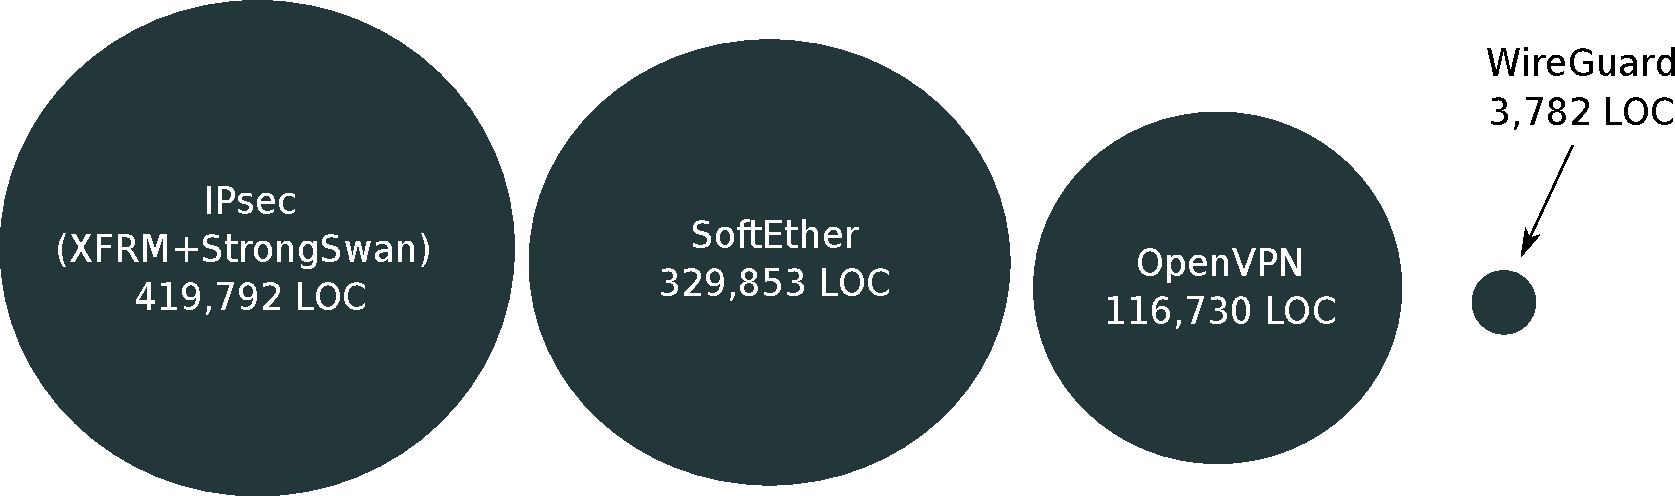
\includegraphics[width=\textwidth]{vpn_compare.pdf}
            \caption{Comparing different VPN protocols in terms of LOC}
        \end{figure}
    \end{frame}
    \begin{frame}[fragile]{Minimialistic Interface}
    ``Developers should write programs that can communicate easily with other programs''
    \\[5pt]
    \rightline{{\rm --- Unix Philosophy}}
        \begin{itemize}
            \item Wireguard presents a normal network interface
                \begin{lstlisting}
# ip link add wg0 type wireguard
# ip address add 10.0.32.1/24 dev wg0
# ip route add default via wg0
                \end{lstlisting}
            \item By using a standard interface it becomes easier to administer using the existing iproute2 utilities for example
        \end{itemize}
    \end{frame}
    \begin{frame}{Cryptokey Routing}
        \begin{itemize}
            \item Fundamental concept of any VPN service
                \begin{itemize}
                    \item Create \textbf{mapping} between \textbf{public keys of peers} and their \textbf{IPs}.
                \end{itemize}
            \item WireGuard interface has:
                \begin{itemize}
                    \item A private key
                    \item A listening UDP port
                    \item A list of peers
                \end{itemize}
            \item Peer has
                \begin{itemize}
                    \item A public key
                    \item A list of associated tunnel IPs
                    \item Optionally has an endpoint IP and port
                \end{itemize}
        \end{itemize}
    \end{frame}
    \begin{frame}[fragile]{Cryptokey Routing}
        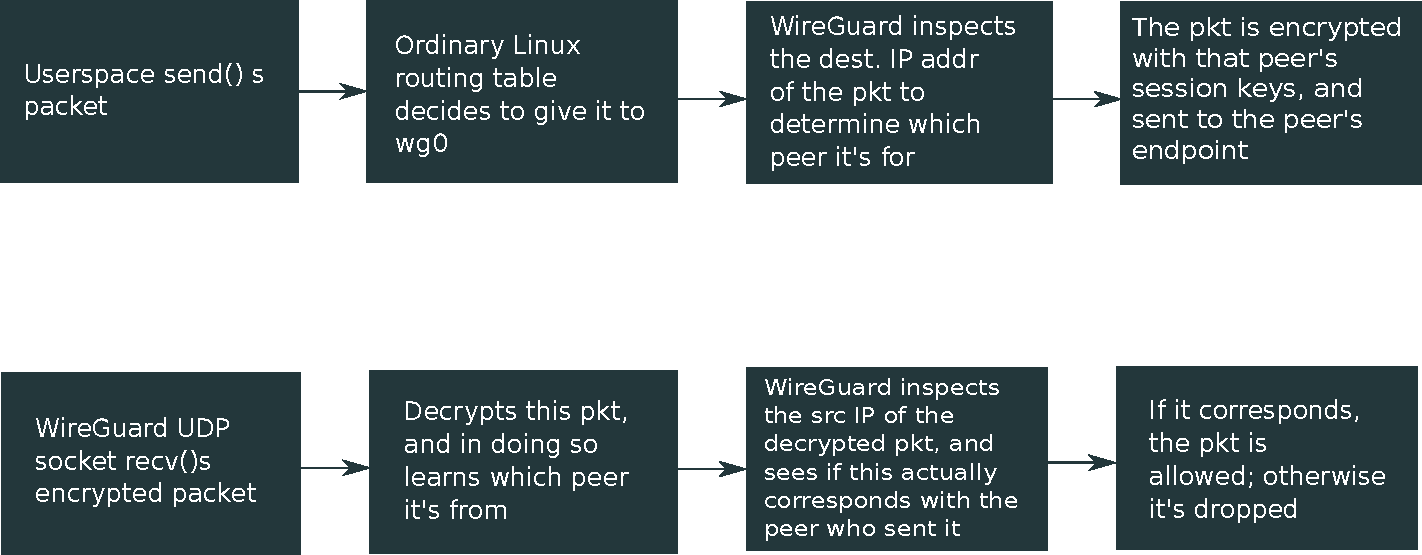
\includegraphics[width=\textwidth]{crypto_route.pdf}
    \end{frame}
    \begin{frame}[fragile]{Performance}
        \begin{figure}
            \hspace*{-1cm} \subfloat{{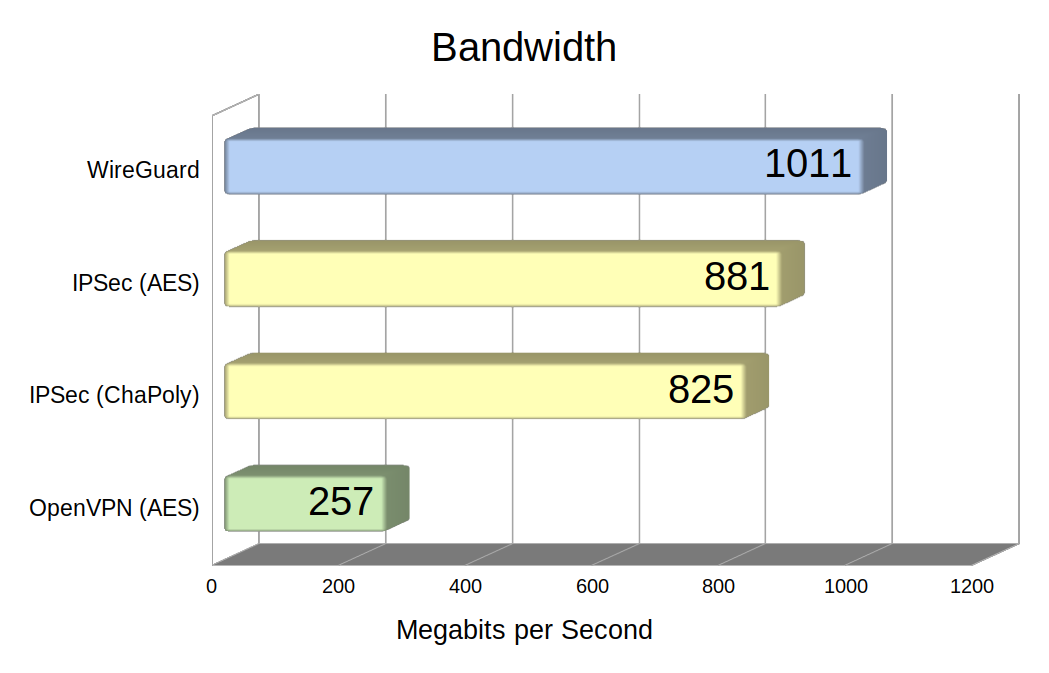
\includegraphics[width=6cm]{bandwidth.png} }}%
            \subfloat{{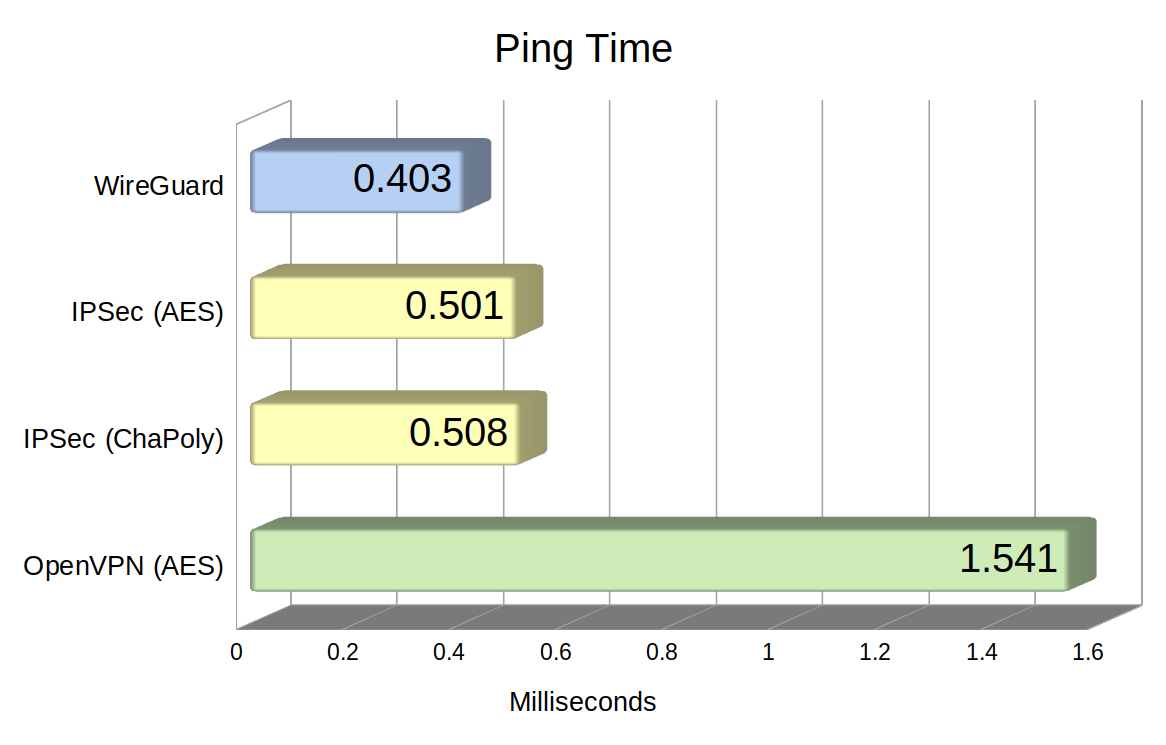
\includegraphics[width=6cm]{ping.png} }}%
            \label{fig:example}%
        \end{figure}
    \end{frame}
    \begin{frame}{Stealth}
        \begin{minipage}{0.6\textwidth}
            \begin{itemize}
                \item Behaves like a rootkit in some sense.
                \item Should not respond to any unauthenticated packets.
                \item Hinder scanners and service discovery.
                \item Service only responds to packets with correct crypto.
                \item Not chatty at all. 
            \end{itemize} 
        \end{minipage}
        \begin{minipage}{0.37\textwidth}
            \begin{figure}
                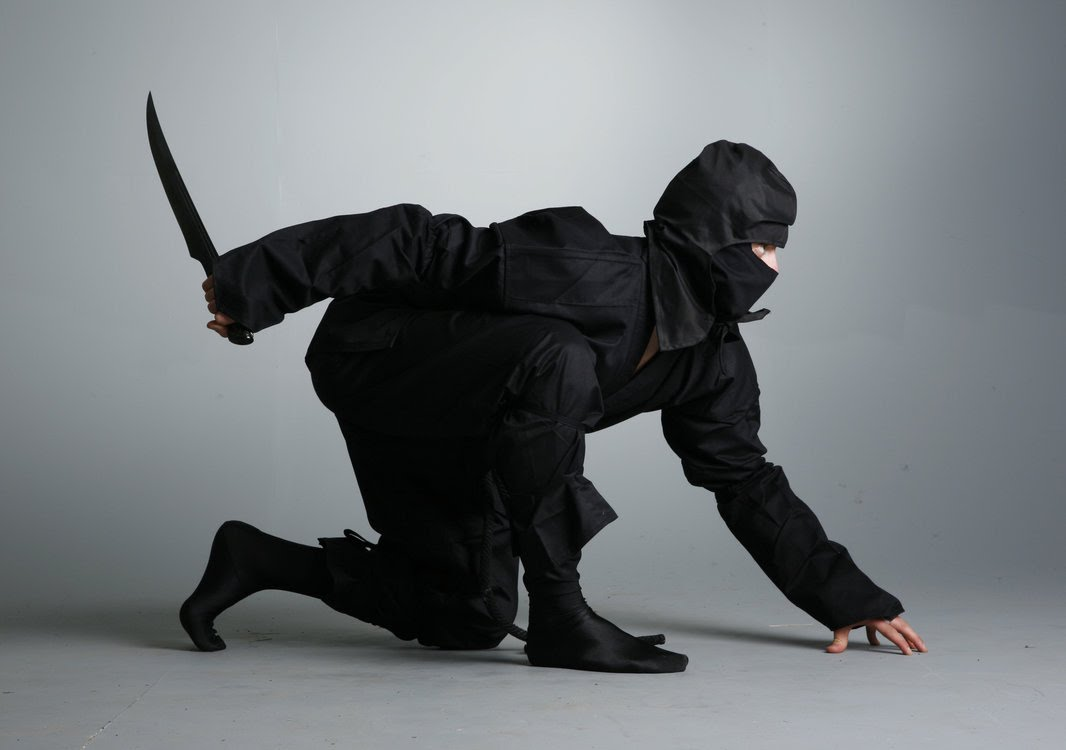
\includegraphics[width=\textwidth]{ninja.jpg}
            \end{figure}
        \end{minipage}
    \end{frame}

    \section{Protocol design}

    \begin{frame}{Handshake DoS}
    \begin{itemize}
        \item Verifying authenticity using Curve25519 is expensive,
        \item Under load a server may send a cookie which needs to be echoed back,
        \item This proves IP ownership, hence IP rate limiting can be used (e.g. token bucket).
        \item The cookie is the MAC over the source IP with a secret which changes every 120s.
    \end{itemize}
    \end{frame}

    \begin{frame}{Flaws to be addressed}
        \begin{itemize}
            \item Indescriminate cookie responses violate silence property,
            \item Cleartext cookies are vulnerable to MiTM replay attacks,
            \item Initator itself could be DoS'ed by being sent fake cookies
        \end{itemize}
    \end{frame}

    \begin{frame}{Issue 1: Silence}
        \begin{itemize}
            \item For the responser to remain silent, all messages have a first MAC using the responder's public key,
            \item This proves that a peer knows to whom it is talking,
            \item While this public key is not secret, it is acceptable in the threat model to say if the initator knows the public key, then it knows of the existance of the server,
            \item This MAC is included in all packets as \texttt{msg.mac1}
        \end{itemize}
    \end{frame}

    \begin{frame}{Issue 2: Cleartext cookies}
    \begin{itemize}
        \item The cookie is encrypted using \texttt{XChaCha20Poly1305 AEAD} with a randomized nonce,
        \item This uses the responders public key as as symmetric encryption key
    \end{itemize}
    \end{frame}

    \begin{frame}{The Key Exchange}
        \begin{figure}
            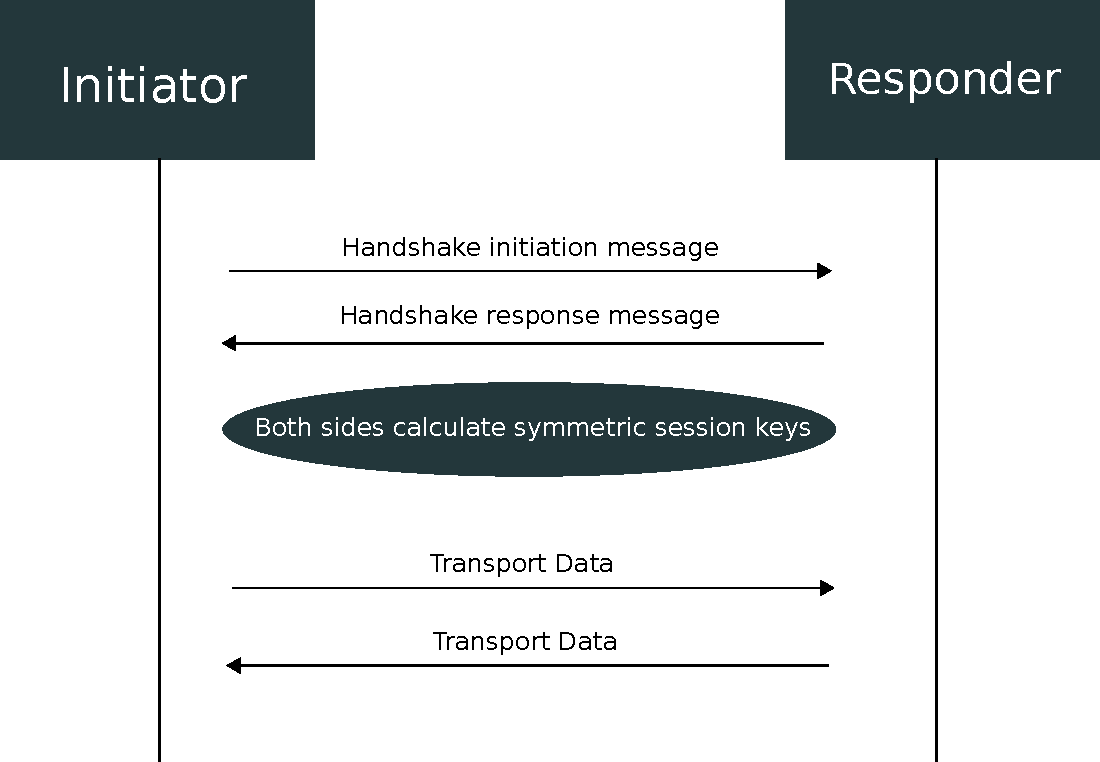
\includegraphics[width=\textwidth]{handshake.pdf}
        \end{figure}
    \end{frame}
    \begin{frame}{Session key derivation - NoiseIK}
        \begin{itemize}
            \item One peer is the initiator; the other is responder
            \item Each peer has their static identity - their long term \textit{static keypair}
            \item For each new handshake, each peer generates an \textit{ephemeral keypair}
            \begin{figure}
                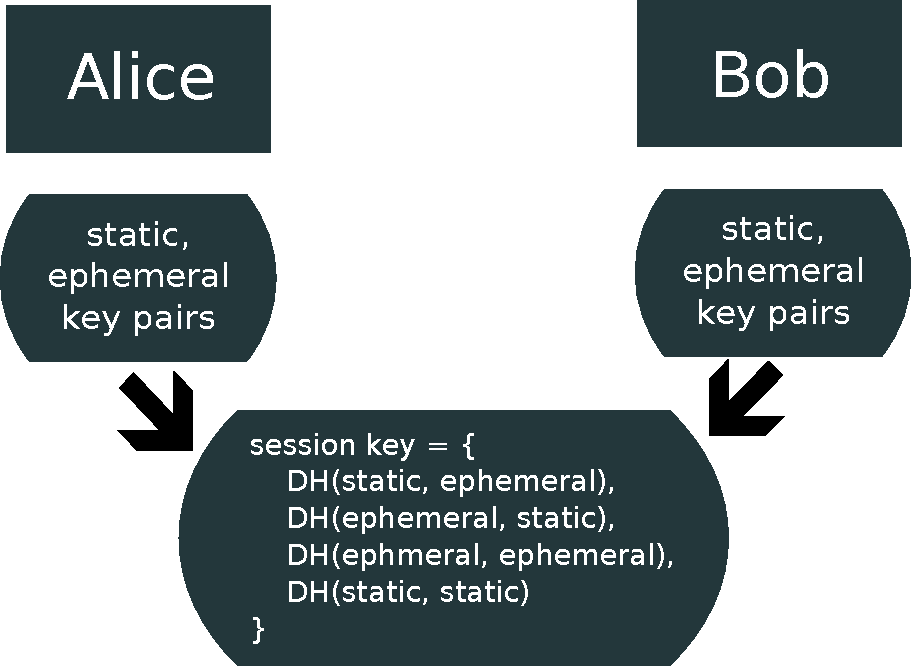
\includegraphics[width=0.6\textwidth]{session_key.pdf}
            \end{figure}
        \end{itemize}
    \end{frame}

    \begin{frame}{Message 1: Initator to responder}
        %XXX Horrific abuse of bytefield to make it look nice.
        \begin{figure}
        \begin{bytefield}{32}
            \bitbox{13}{Type := 1 (1 byte)}
            \bitbox{19}{Reserved := 0 (3 bytes)}\\
            \bitbox{32}{Sender := $I_i$ (4 bytes)}\\
            \wordbox{1}{Ephemeral (32 bytes)}\\
            \wordbox{1}{Static (32 bytes)}\\
            \wordbox{1}{Timestamp (12 bytes)}\\
            \bitbox{16}{mac1 (16 bytes)}
            \bitbox{16}{mac2 (16 bytes)}
        \end{bytefield}
        \caption{Initator to responder packet. \tiny{\textsc{not to scale}}.}
        \end{figure}
    \end{frame}
    \begin{frame}{Message 2: Responder to initiator}
        \begin{figure}
        \begin{bytefield}{32}
            \bitbox{13}{type := 0x2 (1 byte)}
            \bitbox{19}{reserved := 0 (3 bytes)}\\
            \bitbox{16}{sender := $I_r$ (4 bytes)}
            \bitbox{16}{receiver := $I_i$ (4 bytes)}\\
            \wordbox{1}{Ephemeral (32 bytes)}\\
            \wordbox{1}{Empty (0 bytes)}\\
            \bitbox{16}{mac1 (16 bytes)}
            \bitbox{16}{mac2 (16 bytes)}\\
        \end{bytefield}
        \caption{Responder to initiator packet. \tiny{\textsc{not to scale}}}
        \end{figure}
    \end{frame}
    \begin{frame}{Transport data messages}
        \begin{figure}
         \begin{bytefield}{32}
            \bitbox{13}{type := 0x4 (1 byte)}
            \bitbox{19}{reserved := 0 (3 bytes)}\\
            \wordbox{1}{receiver := $I_{m'}$ (4 bytes)}\\
            \wordbox{1}{counter (8 bytes)}\\
            \wordbox[lrt]{1}{packet data}\\
            \skippedwords\\
            \wordbox[lrb]{1}{}\\
        \end{bytefield}
        \caption{Payload packet. \tiny{\textsc{not to scale}}}
        \end{figure}
    \end{frame}
\end{document}

